\documentclass{report}
\usepackage[margin=1in]{geometry} 
\usepackage{amsmath,amsthm,amssymb,amsfonts}
\usepackage{tabto}
\usepackage[yyyymmdd]{datetime}
\renewcommand{\dateseparator}{--}
\newcommand{\N}{\mathbb{N}}
\newcommand{\Z}{\mathbb{Z}}

\usepackage{arydshln} % gives hdashline and cdashline
\newcommand*{\tempb}{\multicolumn{1}{:c}{}} % Used for block matrices


% For clickable TOC
\usepackage{hyperref}
\hypersetup{
	colorlinks,
	citecolor=black,
	filecolor=black,
	linkcolor=black,
	urlcolor=black
}

% For definitions
%\newtheorem{defn}{Definition}[section]
%\newtheorem{thrm}{Theorem}[section]
%\newtheorem{ex}[Example}[section]
\theoremstyle{plain}
\newtheorem*{thrm}{Theorem}
\newtheorem*{lemma}{Lemma}

\theoremstyle{definition}
\newtheorem*{ex}{Example}
\newtheorem*{defn}{Definition}
\newtheorem*{result}{Result}

\theoremstyle{plain}

% For circled text
\usepackage{tikz}
\newcommand*\circled[1]{\tikz[baseline=(char.base)]{
            \node[shape=circle,draw,inner sep=0.8pt] (char) {#1};}}

% For equation system alignment
\usepackage{systeme,mathtools}
% Usage:
%	\[
%	\sysdelim.\}\systeme{
%	3z +y = 10,
%	x + y +  z = 6,
%	3y - z = 13}

\newenvironment{problem}[2][Problem]{\begin{trivlist}
\item[\hskip \labelsep {\bfseries #1}\hskip \labelsep {\bfseries #2.}]}{\end{trivlist}}
%If you want to title your bold things something different just make another thing exactly like this but replace "problem" with the name of the thing you want, like theorem or lemma or whatever
 
%used for matrix vertical line
\makeatletter
\renewcommand*\env@matrix[1][*\c@MaxMatrixCols c]{%
  \hskip -\arraycolsep
  \let\@ifnextchar\new@ifnextchar
  \array{#1}}
\makeatother 
 
% Change chapter numbering
\newcommand{\mychapter}[2]{
	\setcounter{chapter}{#1}
	\setcounter{section}{0}
	\chapter*{#2}
	\addcontentsline{toc}{chapter}{#2}
}


\usepackage{graphicx}
\graphicspath{ {Images/} }
\begin{document}

\mychapter{1}{2018-05-09}
\section{Possible Essay Question}
You have unlimited funding and the ultimate peripheral device and you're going to build an intelligent. Will you have any neural component in the device? If so, justify.

\section{TLU}
TLU - Threshold Logic Unit\\
\begin{center}
\centering
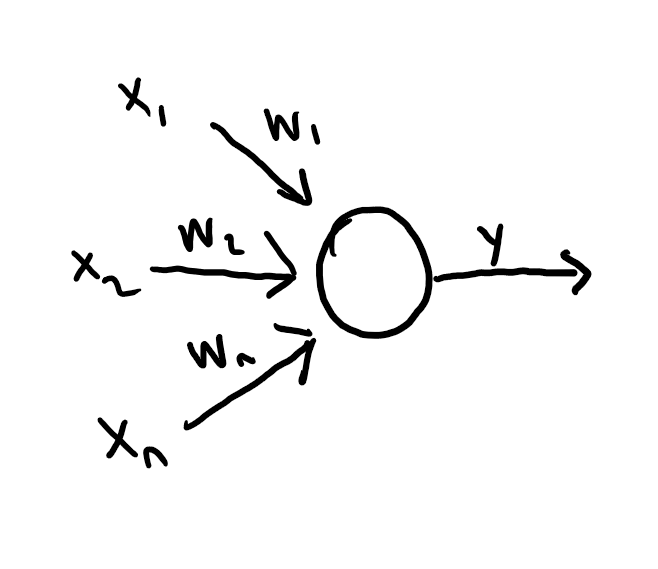
\includegraphics[width=0.25\textwidth]{McColloch-Pitts-Neuron}\\
Above is a McColloch-Pitts neuron where the following hold:
\end{center}
\begin{align}
x &\in \{0,1\}\\
y&=\left\{\begin{array}{cc}0 & \sum_i x_i-w_i \geq 0\\1 & \pi\\\end{array} \right.\\
w &\in \mathbb{R}
\end{align}

\section{Gradient Descent}
Our goal in gradient descent is to find the partial derivative $\dfrac{\partial E}{\partial W}$. Gradient descent is assuming that there is a relation between the errors and the weights. We are looking for the minima in this function.
\[ \Delta w = \dfrac{\partial E}{\partial w} \]

\section{Perceptron Learning Algorithm}
Using the same neuron design as before, we follow the steps below:
\begin{enumerate}
\item Input $\bar{x}$ which is a vector of inputs.
\item Output $y$
\item Compute to target $\hat{y}$
\end{enumerate}

Suppose $y=0,\hat{y}=1$, add $\Delta$ to reach the expected value.\\
This algorithm draws a hyperplane through the function and classifies based on what side of the line each value is. 
\end{document}